\section{Le Perceptron}
\fancyhead[R]{\textit{\nouppercase{\leftmark}}}

\subsection{Modèle du perceptron}

Le perceptron est un des algorithmes de base du machine learning. Son invention remonte aux années 70, mais l'algorithme a été abandonné en 
raison de son exécution trop coûteuse pour les performances des ordinateurs de l’époque. Ce n’est que récemment qu’il a pu resurgir, grâce 
à l’amélioration des processeurs et des cartes graphiques, particulièrement adaptées aux calculs matriciels.

Le modèle du neurone est le suivant : 

\begin{figure}[h]
 \centering
 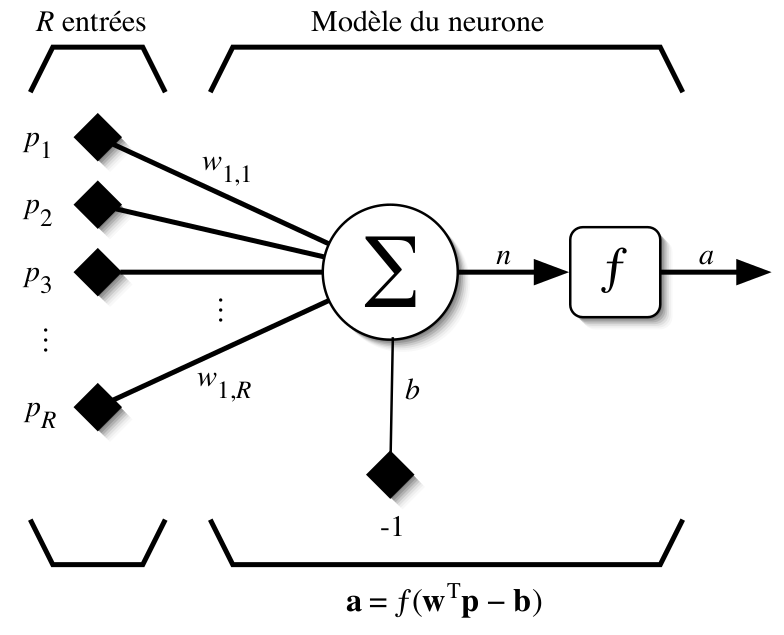
\includegraphics[width=0.5\textwidth]{img/neurone.png}
 \caption{Modèle d'un neurone artificiel}
\end{figure}

Le neurone est composé de différents élements : 
\begin{itemize}
 \item $p_1$, $p_2$, ..., $p_R$ constituent les $R$ variables d'entrées du perceptron. Le nombre d'entrées est souvent imposé par le système lui-même.
 \item $w_{1,1}$, $w_{1,2}$, ..., $w_{1,R}$ sont les poids associés respectivement à chaque entrée. Ils mesurent l'importance accordée à chaque entrée. Un poids
 plus important signifie que l'entrée associée est plus pertinente pour ce neurone que les autres.
 \item Le biais $b$
 \item Le niveau d'activation $n$
 \item La fonction d'activation $f$
 \item La sortie $a$
\end{itemize}

Ainsi, on associe les entrées et les poids par un produit scalaire, pour en sortir une valeur qui caractérise l'entrée, le niveau d'activation.
On ajoute un biais pour régler l'importance accordée au niveau d'activation. On peut utiliser une notation matricielle pour simplifier les calculs.
On pose alors $\mathbf{w_1} = 
\begin{pmatrix}
  w_{1,1} & w_{1,2} & \ldots & w_{1,R}\\
\end{pmatrix}^T $ 
et
$ \mathbf{p} = 
\begin{pmatrix}
 p_1 & p_2 & \ldots & p_R \\
\end{pmatrix}^T $, 
les vecteurs colonnes représentant respectivement les entrées et les poids du neurone. On a alors :

\begin{equation} 
n = \sum_{i=1}^{R} w_{1,i} p_i - b = \mathbf{w_1}^T \mathbf{p} - b
\end{equation}

On cherche alors à discriminer les différentes possibilités pour le niveau d'activation. C'est le rôle de la fonction d'activation. Si l'on souhaite séparer
le cas d'un $n$ supérieur ou non à un seuil donné, alors on utilise la fonction seuil $ f : x \mapsto \mathds{1}_{n \geq 0} $. On remarquera qu'il n'est 
pas nécessaire de changer le seuil de la fonction car c'est le rôle incarné par le biais. Néanmoins, d'autres fonctions peuvent être utilisées à la place
du seuil telles que la sigmoide ($\sigma : x \mapsto \frac{1}{1+e^{-x}}$) ou encore la tangente hyperbolique. 
On préfère généralement des fonctions différentiables pour permettre au réseau d'apprendre sur les données fournies.

On a alors : 
\begin{equation}
 a = f\left(\mathbf{w_1}^T \mathbf{p} - b\right)
\end{equation}

Si on revient au cas de la fonction seuil, on remarquera qu'elle permet de séparer le plan en deux espaces : l'un où la sortie est nulle, l'autre où
la sortie est égale à 1. Puisque le niveau d'activation résulte d'un produit matriciel, cela définit l'équation d'un hyperplan, la séparation
est donc linéaire.

\begin{figure}[h]
 \centering
 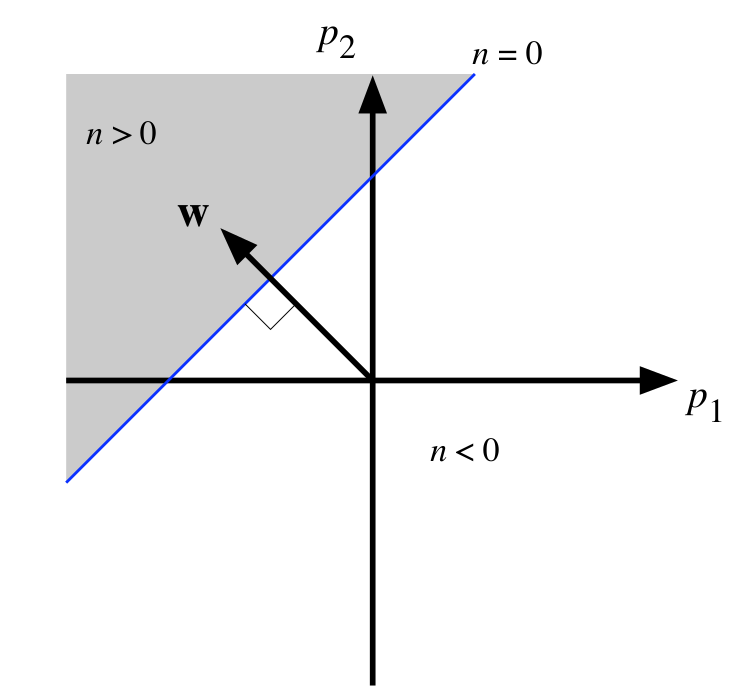
\includegraphics[width=0.5\textwidth]{img/separation_lineaire_du_plan.png}
 \caption{Domaine de séparation du neurone}
\end{figure}

Ce neurone n'est capable de traiter que les données qui peuvent être séparées linéairement (par un hyperplan). Pour des jeux de données plus complexes,
on a parfois besoin de définir des ensembles plus élaborés.
Pour cela on utilise plusieurs neurones sur une même couche. Tous les neurones reçoivent la même entrée, mais chacun possède ses propres poids et son propre biais.
Ainsi, chaque neurone de la couche définit un hyperplan de séparation des données. On peut alors à nouveau représenter le modèle de manière matricielle.
Un vecteur de sortie définit les différentes valeurs des neurones, une matrice de poids définit les poids pour chaque neurone (à chaque neurone est associée
une ligne de la matrice). De la même manière, on retrouve un vecteur de biais (qui sont essentiellement des poids dont l'entrée est constante à $-1$), et 
un vecteur de niveaux d'activation. Finalement, on retrouve ce modèle : 

\begin{figure}[h]
 \centering
 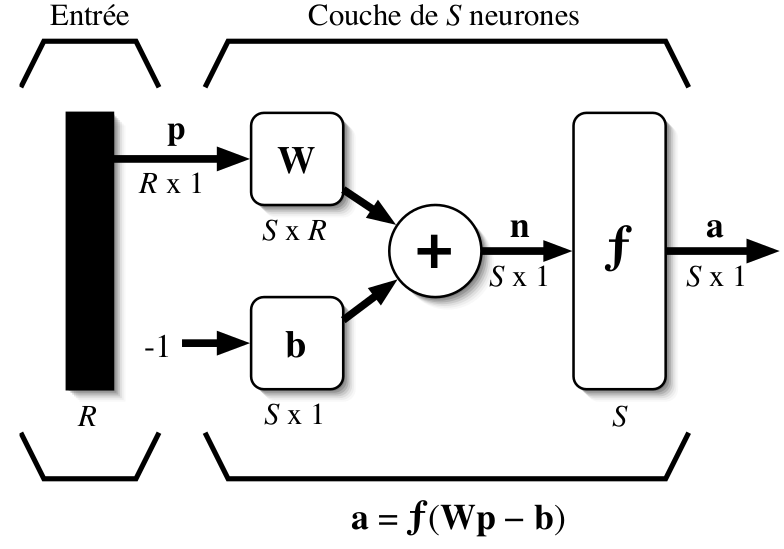
\includegraphics[width=0.55\textwidth]{img/couche.png}
 \caption[Modèle d'une couche de neurones]{Représentation matricielle d'une couche de S neurones recevant R entrées}
\end{figure}

Pour pouvoir définir des ensembles de solutions plus complexes, on ajoute d'autres couches de neurones. Chaque couche prend en entrée le vecteur de sortie
de la couche qui la précède. Cela permet donc de traiter les différents hyperplans de la première couche, et de les lier (par exemple pour en faire
l'intersection). Ainsi, avec deux couches, le réseau peut représenter n'importe quel ensemble convexe. Une troisième couche permet de représenter des
ensembles non convexes.

\begin{figure}[h]
 \centering
 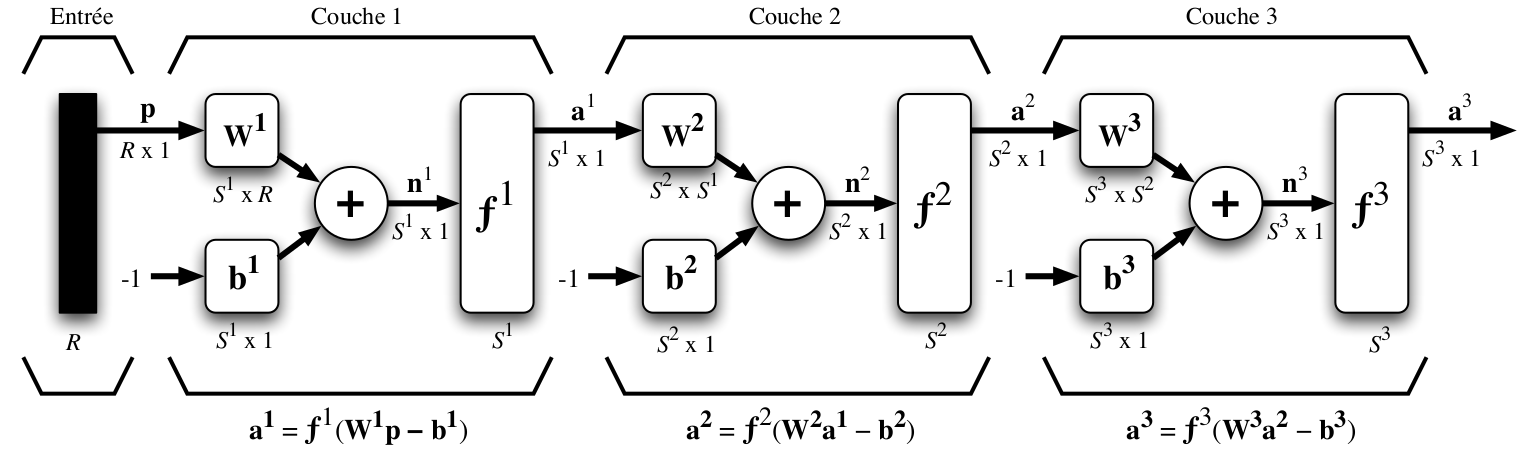
\includegraphics[width=\textwidth]{img/modele_perceptron_multicouches.png}
 \caption{Modèle du perceptron multicouches}
\end{figure}


\subsection{Apprentissage}

L'intérêt du modèle serait limité s'il devait être calculé manuellement. L'objectif est d'avoir un algorithme qui trouve lui-même les paramètres du réseau
(poids et biais) pour s'adapter à un jeu de données collectées au préalable. Il existe plusieurs méthodes pour réaliser l'apprentissage. Dans le cas du 
perceptron, on utilise souvent un apprentissage supervisé. Cela signifie que les données collectées contiennent la ``bonne'' réponse pour que 
le réseau puisse apprendre en conséquence. D'autres méthodes comme l'apprentissage non supervisé existent, ce dernier reposant uniquement sur les jeux 
d'entrées ; dans ce cas, le réseau doit les discriminer lui-même sans connaître la ``bonne'' réponse.

Pour réaliser cela, on présente à notre réseau une entrée ; dans la mesure où l'on dispose de la sortie attendue, il est possible de quantifier l'erreur
faite par le réseau.
C'est le rôle de la fonction d'erreur. Plus celle-ci est importante, moins le réseau est adapté pour cette donnée. Il existe différentes fonctions
d'erreur. Une des plus utilisées est la somme des carrés des écarts entre la valeur attendue et la valeur calculée : 

\begin{equation}
\displaystyle F\left(\mathbf{x}\right) = \mathbf{e\left(x\right)}^T\mathbf{e\left(x\right)} 
\end{equation}

où $\displaystyle \mathbf{e\left(x\right)} = \mathbf{d\left(x\right)} - \mathbf{a\left(x\right)} $,
$\mathbf{d\left(x\right)}$ la valeur attendue et $\mathbf{a\left(x\right)}$ la valeur calculée.


L'apprentissage consiste donc en la minimisation de cette fonction de coût $F$. À chaque calcul d'erreur, on modifie les différents poids du réseau.
À une couche $k$ donnée, le poids entre l'entrée $j$ et le neurone $i$ est modifié de la manière suivante : 
\begin{equation}
 \Delta w^k_{i,j}\left(t\right) = - \eta \frac{\partial F}{\partial w^k_{i,j}}
\end{equation}
 
En se plaçant dans l'espace des poids (cela inclut les biais qui sont des poids particuliers), cela revient à chercher la direction dans laquelle l'erreur
est diminuée de la manière la plus significative. Le facteur $\eta$ est le taux d'apprentissage (Learning Rate en anglais). Il représente le pas de
chaque itération vers le minimum de la fonction de coût. C'est un paramètre du réseau que nous devons choisir en amont de l'apprentissage.

Marc \textsc{Paruzeau} démontre en 2004 les formules de rétropropagation que nous avons utilisées. Pour cela il introduit un paramètre % pas vraiment un paramère quand pensez-vous ? je ne trouve aps le mot juste
intermédiaire. Les sensibilités sont définies ainsi :
\begin{equation}
 \mathbf{s}^k = \frac{\partial F}{\partial \mathbf{n}^k}
\end{equation}

On note également l'utilisation du raccourci suivant : 

\begin{equation}
  \displaystyle
 \mathbf{\dot F}^k\left(\mathbf{n}^k\right) =
 \begin{bmatrix}
  \dot f ^k\left(n^k_1\right) & 0 & \ldots & 0\\
  0 & \dot f^k\left(n^k_2\right) & 0 & 0\\
  \vdots & \vdots & \ddots & \vdots \\
  0 & 0 & \ldots & \dot f^k\left(n^k_{S^k}\right)\\
 \end{bmatrix}
 \text{où $S^k$ est le nombre de neurones de la couche $k$}
\end{equation}

Pour un réseau de $M$ couches, la rétropropagation se déroule de la manière suivante~:
\begin{itemize}
 \item On propage notre entrée $\mathbf{p}$ dans le réseau
 \begin{equation}
   \mathbf{a}^k = \mathbf{f}^k\left(\mathbf{W}^k\mathbf{a}^{k-1} - \mathbf{b}^k\right) \text{, pour $k \in \intervalle{\llbracket}{1}{M}{\rrbracket}$ et $\mathbf{a}^0 = \mathbf{p}$}
 \end{equation}
 
 \item On calcule les sensibilités 
 \begin{align}
  \mathbf{s}^M &= -2\mathbf{\dot F}^M\left(\mathbf{n}^M\right)\mathbf{e} \\
  \mathbf{s}^k &= \mathbf{\dot F}^k\left(\mathbf{n}^k\right)\left(\mathbf{W}^{k+1}\right)^T \mathbf{s}^{k+1} \text{, pour $k \in \intervalle{\llbracket}{1}{M-1}{\rrbracket}$}
 \end{align}
 
 \item On calcule les changements de poids
 \begin{align}
  \Delta \mathbf{W}^k &= - \eta \mathbf{s}^k\left(\mathbf{a}^{k-1}\right)^T \text{, pour $k \in \intervalle{\llbracket}{1}{M}{\rrbracket}$} \\
  \Delta \mathbf{b}^k &= \eta \mathbf{s}^k \text{, pour $k \in \intervalle{\llbracket}{1}{M}{\rrbracket}$}
 \end{align}

\end{itemize}

\subsection{La fonction d'erreur}

Puisque l'on réalise un apprentissage supervisé, on suppose qu'à chaque jeu de données, on connaît la sortie attendue. Il est alors nécessaire
de mesurer l'erreur entre la sortie attendue et la sortie calculée par le réseau neuronal.

Il existe plusieurs formulations de cette erreur, telles que l'erreur quadratique (norme euclidienne du vecteur d'erreur), l'erreur moyenne (norme 1 du vecteur d'erreur)... 
Pour obtenir l'erreur d'un groupe de données (batch), on somme les erreurs de chaque données. Par soucis de simplicité, nous avons décidé d'utiliser
l'erreur quadratique pour notre perceptron. Néanmoins il existe une autre fonction d'erreur : l'entropie croisée. Nous allons voir dans ce rapport pourquoi 
cette fonction possède de meilleures propriétés que l'erreur quadratique.

La formule de l'entropie croisée est la suivante : 
\begin{equation}
 C = -\frac{1}{n}\sum_x\left(y\ln\left(a\right) + \left(1-y\right)\ln\left(1-a\right)\right)\; \text{, \parbox[t]{15em}{$n$ la taille du batch\\ $x$ les exemples du batch\\
 $a$ la sortie calculée\\$y$ la sortie attendue}}
 \label{eq:formule-entropiecroisee}
\end{equation}

\subsubsection{Comportement pour une erreur quadratique}

Pour comprendre l'intérêt de cette formule, nous devons comprendre pourquoi la norme euclidienne échoue. Le concept d'entropie provenant 
directement de la théorie des probabilités, on doit donc choisir judicieusement la fonction d'activation de notre couche de sortie. On 
considère souvent que l'entropie correspond naturellement à une fonction d'activation de sortie de type sigmoïde. 

Pour simplifier le raisonnement, nous utilisons un réseau neuronal trivial (un neurone à une entrée et une sortie) de fonction d'erreur quadratique. 
Néanmoins, les phénomènes observés sur ce neurone unique restent vrais pour des réseaux plus complexes. On dispose donc d'un neurone, avec une entrée (et un biais) et 
une sortie, auquel on souhaite apprendre le comportement suivant~: lorsque l'entrée vaut 1, la sortie doit valoir 0.
Les poids du neurone sont initialisés de manière aléatoire. D'après la figure \ref{fig:initialisation1-entropiecroisee-schema}, on a après initialisation 
un neurone qui renvoit 0.82 lorsque l'entrée vaut 1. On entraîne ce neurone et obtient la courbe d'apprentissage 
\ref{fig:initialisation1-entropiecroisee-courbe}.


\begin{figure}[h]
\centering
\begin{subfigure}{.5\textwidth}
  \centering
  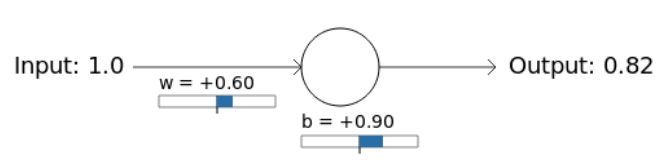
\includegraphics[width=.6\linewidth]{img/entropiecroisee_reseau_utilise.png}
  \caption{Réseau utilisé et son initialisation}
  \label{fig:initialisation1-entropiecroisee-schema}
\end{subfigure}%
\begin{subfigure}{.4\textwidth}
  \centering
  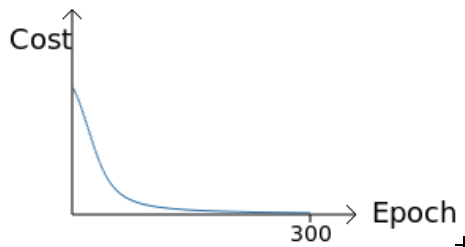
\includegraphics[width=.4\linewidth]{img/entropiecroisee_apprentissage1.png}
  \caption{Courbe d'apprentissage du neurone}
  \label{fig:initialisation1-entropiecroisee-courbe}
\end{subfigure}
\caption{Première initialisation du réseau d'exemple utilisant l'erreur quadratique}
\label{fig:initialisation1-entropiecroisee}
\end{figure}


Sur la courbe \ref{fig:initialisation1-entropiecroisee-courbe}, 
on ne pose pas de valeur concernant le coût. En effet, les informations pertinentes de cette courbe ne sont pas les valeurs initiales 
et finales (augmenter le nombre d'itérations permettrait de réduire cela de manière arbitrairement faible). On s'intéresse plutôt à l'allure générale de 
la courbe. L'apprentissage sur cet exemple est très satisfaisant. 

On considère maintenant un second exemple. Le même réseau est utilisé, mais avec 
une initialisation différente, de sorte que la sortie soit plus proche de 1. On est donc plus éloigné de l'objectif, puisque l'on cherche à retrouver 0.
Les données et résultats de cet exemple sont illustrés par la figure \ref{fig:initialisation2-entropiecroisee-courbe}.
On remarque que l'apprentissage est de qualité moindre. En effet, juste après l'initialisation, le neurone commettait une erreur plus importante,
mais l'apprentissage est beaucoup plus lent. On doit donc réaliser un nombre d'itérations supérieur pour retrouver le cas
\ref{fig:initialisation1-entropiecroisee} et pouvoir apprendre correctement.

\begin{figure}[h]
\centering
\begin{subfigure}{.5\textwidth}
  \centering
  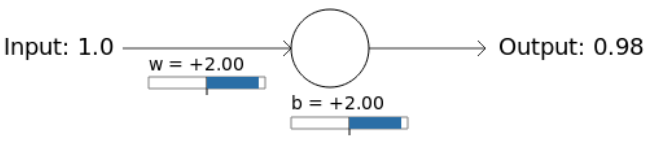
\includegraphics[width=.6\linewidth]{img/entropiecroisee_reseau_utilise_init2.png}
  \caption{Réseau utilisé et son initialisation}
  \label{fig:initialisation2-entropiecroisee-schema}
\end{subfigure}%
\begin{subfigure}{.4\textwidth}
  \centering
  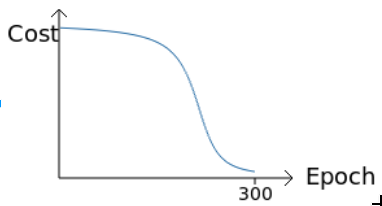
\includegraphics[width=.4\linewidth]{img/entropiecroisee_apprentissage2.png}
  \caption{Courbe d'apprentissage du neurone}
  \label{fig:initialisation2-entropiecroisee-courbe}
\end{subfigure}
\caption{Seconde initialisation du réseau d'exemple utilisant l'erreur quadratique}
\label{fig:initialisation2-entropiecroisee}
\end{figure}

\subsubsection{Origine de cet échec}

Puisque $C = \frac{(y-a)^2}{2}$, on peut vérifier que l'on a :
\begin{align}
 \frac{\partial C}{\partial \omega} &= \left(a-y\right)\sigma'\left(z\right)x \text{, \parbox[t]{15em}{où $z$ est l'antécédant de $a$ par la fonction d'activation}}\\
 \frac{\partial C}{\partial b} &= \left(a-y\right)\sigma'\left(z\right) 
\end{align}

En observant la fonction sigmoïde représentée sur la figure \ref{fig:sigmoid_function}, on se rend compte que le problème provient de $\sigma'\left(z\right)$.
En effet, la seconde initialisation ayant une erreur initiale très importante ($a$ proche de 1), on se retrouve dans la 
partie droite de la courbe, où la pente est très faible. Cela provient du fait que $\sigma'\left(z\right) = a\left(1-a\right)$.

\begin{figure}[h]
 \centering
 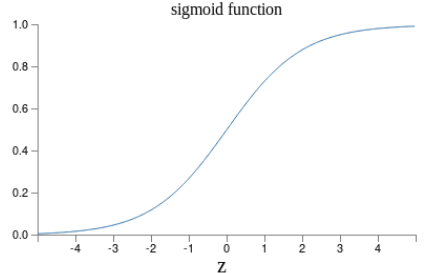
\includegraphics[width=0.3\textwidth]{img/sigmoid_function.png}
 \caption{Graphe de la fonction sigmoïde}
 \label{fig:sigmoid_function}
\end{figure}

\subsubsection{Une solution à ce problème d'apprentissage}
\label{subsubsection:etablissement-eq-entropiecroisee}

L'apprentissage n'en est que ralenti, ce qui n'est évidemment pas souhaitable. Pour rendre le réseau moins sensible à une mauvaise initialisation,
il faut donc changer ce comportement. A nouveau, cela revient à utiliser une analogie avec le comportement humain, puisque l'humain a tendance à apprendre
plus vite lorsque il commet de fortes erreurs. On veut donc garder un apprentissage plus lent lorsque l'on se rapproche du minimum de la fonction
d'erreur. Ainsi, on aimerait obtenir ces équations :

\begin{align}
  \label{eq:comportementvoulu-poids}
  \frac{\partial C}{\partial \omega} &= \left(a-y\right)x \\
  \frac{\partial C}{\partial b} &= \left(a-y\right)
  \label{eq:comportementvoulu-biais}
\end{align}

La formule de la chaîne nous donne 
\begin{equation}
 \frac{\partial C}{\partial b} = \frac{\partial C}{\partial a} \frac{\partial a}{\partial b} = \frac{\partial C}{\partial a} a\left(1-a\right)
\end{equation}

En utilisant l'expression voulue (équation \ref{eq:comportementvoulu-biais}), on obtient 
\begin{align}
 \frac{\partial C}{\partial a} &= \frac{a-y}{a\left(1-a\right)} = \frac{-y}{a} + \frac{1-y}{1-a} \\
 C &= -y\ln\left(a\right) - \left(1-y\right)\ln\left(1-a\right) + Const
\end{align}

On comprend alors que la formule de l'entropie croisée n'est pas simplement une formule qui se trouve avoir des propriétés intéressantes, mais que l'on peut
construire cette fonction de coût pour respecter les conditions des équations \ref{eq:comportementvoulu-poids} et \ref{eq:comportementvoulu-biais}. 
L'expression \ref{eq:formule-entropiecroisee} est alors une condition suffisante et quasiment nécessaire au respect desdites contraintes. 
Le ``quasiment'' provient de la constante d'intégration. Puisque ce n'est pas la fonction de coût en elle-même qui est intéressante mais plutôt
ses variations et ses dérivées partielles, alors on peut se contenter d'une constante nulle, ce qui conserve la positivité de $C$. On s'attend alors
à une amélioration considérable de l'apprentissage observé figure \ref{fig:initialisation2-entropiecroisee}. La courbe d'apprentissage
\ref{fig:initialisation3-entropiecroisee-courbe} montre effectivement un comportement beaucoup plus intéressant. La pente à l'origine est bien plus importante
lorsque le réseau commet une forte erreur. On a ainsi un réseau moins sensible à l'initialisation et qui apprend d'autant plus qu'il commet une
erreur importante. Ce comportement est parfois obtenu en faisant varier le taux d'apprentissage au cours du temps. Sur ces exemples, le taux d'apprentissage
est constant. Ce comportement souhaité étant un artéfact de la fonction de coût, on s'attend à des performances supérieures de la part des réseaux
utilisant l'entropie croisée.

\begin{figure}[h]
\centering
\begin{subfigure}{.5\textwidth}
  \centering
  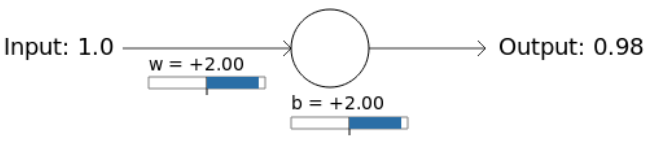
\includegraphics[width=.6\linewidth]{img/entropiecroisee_reseau_utilise_init2.png}
  \caption{Réseau utilisé et initialisation identique à la figure \ref{fig:initialisation2-entropiecroisee}}
  \label{fig:initialisation3-entropiecroisee-schema}
\end{subfigure}%
\begin{subfigure}{.4\textwidth}
  \centering
  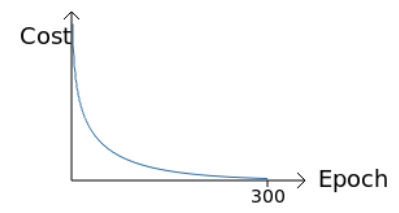
\includegraphics[width=.4\linewidth]{img/entropiecroisee_apprentissage3.png}
  \caption{Courbe d'apprentissage du neurone}
  \label{fig:initialisation3-entropiecroisee-courbe}
\end{subfigure}
\caption{Seconde initialisation du réseau d'exemple en utilisant l'entropie croisée}
\label{fig:initialisation3-entropiecroisee}
\end{figure}

\subsubsection{Une explication intuitive}

La section \ref{subsubsection:etablissement-eq-entropiecroisee} a permis de trouver par le calcul la formule \ref{eq:formule-entropiecroisee}.
On cherche cette fois à obtenir une explication plus intuitive pour mieux comprendre pourquoi cette fonction de coût est pertinente.

La formule de l'entropie d'une variable aléatoire $X$ est une somme sur les éventualités non improbables :
\begin{equation}
 H(X) = -\sum_{i=1}^{n} p_i\log\left(p_i\right)
\end{equation}

L'entropie est une mesure de l'incertitude d'une loi de probabilité. Par exemple, si on réalise une expérience de boules et que l'on considère
la couleur de la boule tirée, alors l'entropie sera maximale lorsque les différentes éventualités sont équiprobables.

En traitement de l'information, cette grandeur permet de coder efficacement les symboles à transmettre. Si on a des symboles équiprobables,
l'entropie est maximale. Dans ce cas, le nombre de bits nécessaires pour définir un symbole avec certitude est $\log_2\left(N\right)$, où $N$ est le nombre
de symboles différents. Cependant, si l'on considère un texte en français, les lettres RSTLNE sont beaucoup plus fréquentes que WXYZ. La diminution de l'entropie
caractérise le fait qu'un système de codage ingénieux utilise en moyenne moins de bits pour transmettre l'information avec certitude.

L'entropie croisée $-p\log\left(q\right)$ est, en mathématiques, une mesure de la distance entre deux distributions $p$ et $q$. On peut là encore y 
retrouver une interprétation dans le domaine du traitement de signal. 
En effet, si on considère un système de codage adapté à un texte dans lequel chaque lettre apparaît selon une distribution $q$, alors
l'entropie croisée $-p\log\left(q\right)$ quantifie l'adaptation de ce même système pour chiffrer un texte dans lequel 
chaque lettre apparaît selon la distribution $p$.

Ainsi, si on dispose d'un jeu de données dont les sorties attendues suivent une distribution empirique $p$, et d'un réseau neuronal dont les sorties
à ces données suivent une distribution $q$, alors adapter le réseau pour qu'il puisse reproduire fidèlement les observations $p$ revient 
à diminuer l'entropie croisée de ces deux distributions.

\subsubsection{Estimateur de l'entropie croisée}

On considère un batch de taille $n$ contenant $N$ données distinctes $\{x_1, x_2, \ldots, x_N\}$, chaque observation $x_i$ 
(pour $i \in \intervalle{\llbracket}{1}{N}{\rrbracket}$) apparaît dans le batch $np_i$ fois.

Notre réseau est alors ainsi constitué : la couche de sortie est composée d'un seul neurone (une somme de l'entropie sur les neurones peut être faite si 
on a une couche de plusieurs neurones) et d'une fonction d'activation sigmoïde donnant une sortie $q_i$ lorsque soumise à l'exemple $x_i$. On a alors :

\begin{equation}
 \mathbb{P}\left(X=y_i\right) = \begin{cases}q_i &\text{ si $y_i=1$}\\1-q_i &\text{ si $y_i=0$}\end{cases} \text{, \parbox[t]{20em}{où $X$ représente notre réseau\\
 et $y_i$ représente l'observation à la donnée $x_i$}}
 \label{eq:proba}
\end{equation}

$\mathbb{P}$, tel que défini par l'équation \ref{eq:proba}, représente la probabilité que notre réseau trouve la bonne solution. Sa densité de probabilité
est donnée sous une forme différente par l'équation \ref{eq:ddp}
\begin{equation}
 \label{eq:ddp}
 \mathbb{P}\left(X=y_i\right) = q_i{^{y_i}}\left(1-q_i\right)^{1-y_i}
\end{equation}

Les équations \ref{eq:vraisemblance} et \ref{eq:log-vraisemblance} ci-dessous présentent respectivement la vraisemblance et la log-vraisemblance de notre loi.

\begin{align}
 \mathbb{L} &= \prod_{i=1}^N q_i{^{np_i}}\left(1-q_i\right)^{n(1-p_i)}
 \label{eq:vraisemblance}\\
 \frac{1}{n}\log\left(\mathbb{L}\right) &= \sum_{i=1}^N \left(p_i\ln\left(q_i\right) + \left(1-p_i\right)\ln\left(1-q_i\right) \right)
 \label{eq:log-vraisemblance}
\end{align}

D'après les équations \ref{eq:formule-entropiecroisee} et \ref{eq:log-vraisemblance}, la log-vraisemblance de notre système est 
ainsi proportionnelle à l'opposé de l'entropie croisée. 
Ainsi, on comprend que minimiser l'entropie croisée revient à utiliser un estimateur de maximum de vraisemblance. 
Notre système est donc d'autant plus performant que son entropie croisée est faible.






\newpage


\subsection{Implémentation}

Afin de pouvoir comprendre en détail le fonctionnement du perceptron, nous avons commencé dans un premier temps à implémenter un version 
de celui-çi chacun de notre côté. Cela nous a permis de commencer  à réfléchir à l’architecture du code que nous voulions, et de pouvoir 
comparer les performances des différentes implémentations. 

Nous avons testé dans un premier temps les résultats de nos perceptrons sur la fonction XOR. Cette fonction est un bon départ pour pouvoir 
avoir un code fonctionnel, car il s’agit d’une fonction ne pouvant pas être répliquée par une fonction linéaire : il faut au moins une couche 
cachée afin de pouvoir l’implémenter grâce à un perceptron. 
Cette prémière étape nous a permis de comparer les résultats et les performances de nos algorithmes, et de pouvoir choisir l’implémentation 
du perceptron que nous avons utilisé par la suite.


\subsection{Résultats}


